%!TEX TS-program = xelatex
%!TEX encoding = UTF-8 Unicode

\documentclass[border=0.0cm]{standalone}
% Pacchetti per font e colori
\usepackage{fontspec}

\usepackage{tikz}

\usepackage{Alegreya}
\usepackage{newpxmath}
%\usepackage{fourier}

\usetikzlibrary{
  decorations.text
}

\begin{document}
\begin{tikzpicture}
  \draw[color=white] (-14.4,-8.2) rectangle (14.4,8.2);
  \tikzstyle{every node}=[font=\small]
  
  \begin{scope}[rotate=3]
%    \draw[very thick] (-5,0) -- (5,0);
%    \draw[very thick, ->] (-3,0) arc (180:2:3cm);
%    \draw[very thick, ->] (3,0) arc (0:-178:3cm);
    
    % Pallino centrale con etichetta
    \draw[fill=black] (0,0) circle (0.1cm);
%    \node[above=3pt, font=\Large] at (0,0) {$m(t)$};
    
    % Pallini superiore e inferiore con etichette
%    \draw[fill=black] (0,3) circle (0.1cm);
%    \node[above=3pt, font=\Large] at (0,3) {FIR};
    
%    \draw[fill=black] (0,-3) circle (0.1cm);
%    \node[below=3pt, font=\Large] at (0,-3) {IIR};
  \end{scope}
  
  \node[anchor=south east] at (13.9,-7) {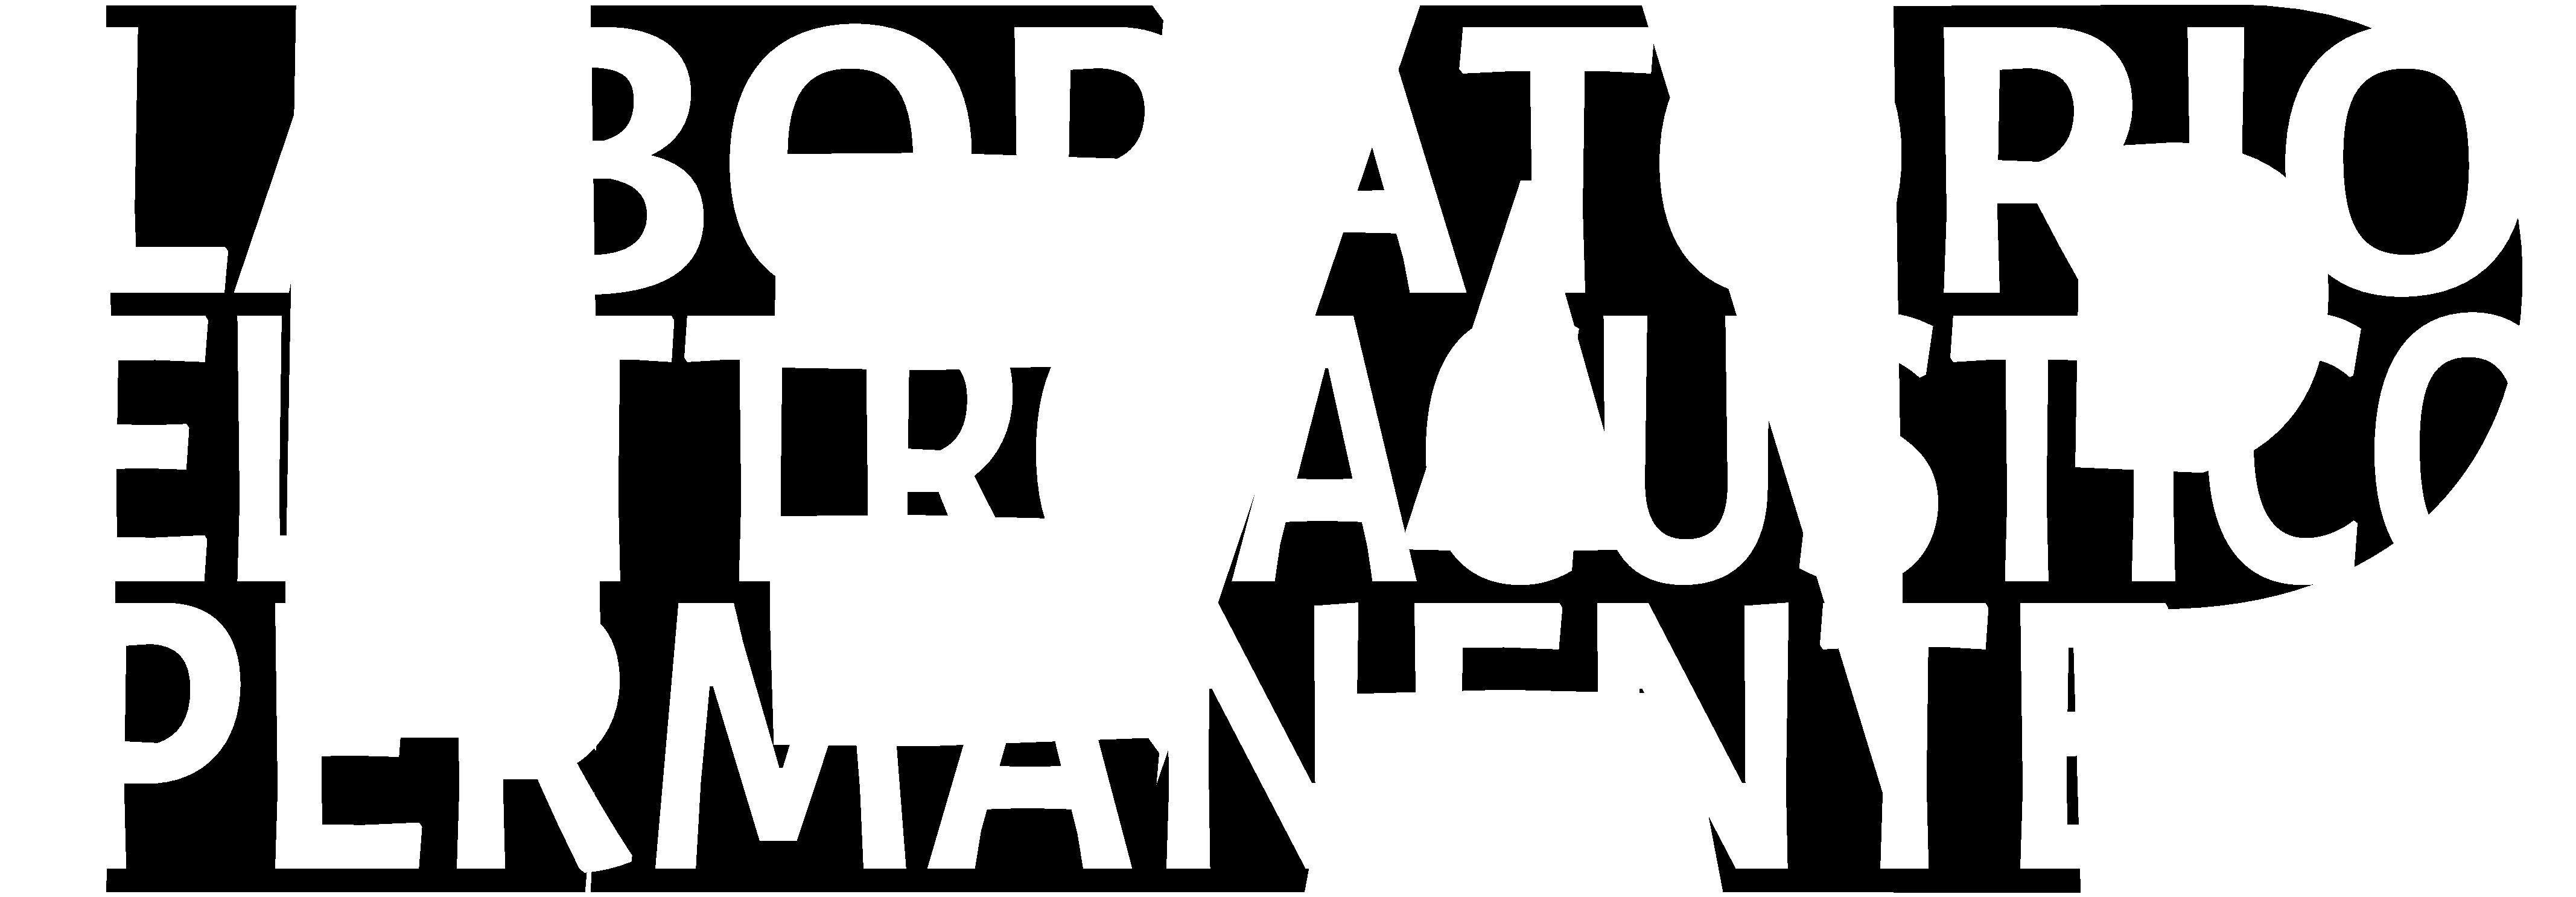
\includegraphics[width=3cm]{2023-11-12-logo-kern.pdf}};
  \node[anchor=south east] at (13.9,-8) {
\includegraphics[width=3cm]{gs-signature_a}};
\end{tikzpicture}
\end{document}

% il punto come entità geometrica ”senza forma e senza dimensione” - solo posizione, senza estensione.

%Significati fondamentali
%La polisemia del termine abbraccia:
%
%Geometrico: entità senza dimensioni che ha solo posizione
%Grafico: segno tipografico (punto fermo, virgola, ecc.)
%Spaziale: luogo determinato ("punto di riferimento")
%Temporale: istante preciso ("a questo punto")
%Argomentativo: questione, tema ("punto di vista")
%Valutativo: unità di misura o valutazione

%Il ragionamento simbolico
%Punto come perforazione → La memoria punge il continuum temporale, fora il flusso dell'esperienza per estrarre frammenti specifici. Come l'ago che perfora il tessuto, la memoria seleziona e isola.
%Punto geometrico → Il ricordo è un'entità senza estensione ma con posizione precisa nel campo della coscienza. Non ha dimensioni proprie, eppure determina coordinate nel nostro spazio interiore.
%Punto spaziale → Ogni memoria è un luogo mentale, un "dove" della psiche. Parliamo infatti di "luoghi della memoria" (loci memoriae della tradizione retorica).
%Punto temporale → Il ricordo cristalliza un istante, lo sottrae al fluire e lo rende presente. È simultaneamente passato (nell'origine) e presente (nell'atto del ricordare).
%Punto argomentativo → Ogni memoria è un punto di vista, una prospettiva specifica sull'esperienza. Non esiste mai il ricordo neutro, ma sempre il ricordo da una posizione.
%La sintesi simbolica
%La memoria, come il punto, è paradossalmente minimale e massimale: infinitamente piccola (l'istante) e infinitamente significativa (l'intero orizzonte di senso che apre).
%Entrambi trasformano la continuità in discontinuità, il flusso in forma, l'indeterminato in determinato.Retry